\documentclass[12pt]{report}

\usepackage[norsk]{babel}
\usepackage{graphicx} % Required for inserting images
\usepackage{graphicx, array, carlito, fancyhdr, comment, etoc, lipsum, enumitem, standalone, subfiles, newclude, float, enumitem, amsmath, hyperref, adjustbox, titlesec, pdfpages}

\usepackage[style=ieee, sorting=none]{biblatex}

% Fjerne Teksten Kapittel fra overskrift. Justerer plasseringen av chapter navn
\titleformat{\chapter}[display]
{\Huge\bfseries}
{}
{-120pt}
{\thechapter.\ }
\titleformat{name=\chapter,numberless}[display]
{\Huge\bfseries}
{}
{-120pt}
{}
\titlespacing*{\chapter}{0pt}{70pt}{10pt} % Juster verdien 40pt for å endre avstanden


%Gir automatisk nytt avsnitt ved linjeskift
\usepackage[parfill]{parskip}

%Ikke inrykk ved nytt avsnitt
\setlength{\parindent}{0pt}

\usepackage{exsheets}
%Vis løsningsforslag på alle oppgaver
\SetupExSheets{solution/print=false}


\usepackage[a4paper, total={6in, 8in}]{geometry}



% Laste inn referanser
\addbibresource{backmatter/referanser.bib}

% Adding abstract funciton
\newcommand{\chapabstract}[1]{
	\begin{quote}
		\singlespacing\small
		\rule{14cm}{1pt}
		#1
		\vskip-4mm
		\rule{14cm}{1pt}
\end{quote}}


% Set up the fancyhdr package
\pagestyle{fancy}
\fancyhf{} % Clear all header and footer fields

% Adjust the footer position
\setlength{\footskip}{3cm} % You can adjust this value as needed

% Define the footer
%\fancyfoot[L]{\vspace{1cm} \makebox[0pt][l]{\hspace{0.5cm} Elektroniske systemer}} % Left-aligned course name, lifted up
\fancyfoot[R]{%
	\begin{minipage}{2cm}
		\centering
		
\includegraphics[height=1cm]{frontmatter/bilder/r171JViZ6gmf8WXujFQw.jpg}\\
%		\vspace{-0.5cm} % Adjust vertical space to center page number
%		\thepage
	\end{minipage}
}
%\fancyfoot[C]{\thepage}

\fancyhead{}
\fancyhead[LE,RO]{\nouppercase{\rightmark}}
\fancyhead[RE,LO]{Side \thepage}





% ------------------    HER STARTER DOKUMENTET   ------------------

\begin{document}
%Setter inn tittelsiden som eksternt dokument
\begin{titlepage}
    \begin{center}
    \vspace*{1cm}
    \Huge
    \textbf{Elektroniske systemer}
    
    \LARGE
    \vspace{0.5cm}
    Øvingsoppgaver for analoge komponenter og måleteknikk i emnet elektroniske systemer

    \vspace{1.5cm}
    \textbf{Carl Magnus Bøe}
    
    2025

\vfill




    
\includegraphics[width=0.6\textwidth]{frontmatter/bilder/r171JViZ6gmf8WXujFQw.jpg}
    \Large
    
    Fagskolen Viken\\
    01TE00F EITKELFH24\\
    Fredrikstad\\

    \end{center}
\end{titlepage}

%Innholdsfortegnelse
\tableofcontents
\chapter{Introduksjon}
\label{ch:introduksjon}
Dette kapittelet inneholder generell informasjon om kompendiet med bakgrunn for arbeidet, oppbygging av dokumentet og lisensinformasjon.

\section{Bakgrunnsinformasjon}
Dette dokumentet er et kompendium som inneholder øvingsoppgaver relevante for delen analoge komponenter i emnet elektroniske systemer. Siden dokumentet blir kontinuerlig revidert, er det datomerkingen på forsiden som angir versjonen av dokumentet. Målet med dette dokumentet er å samle alle øvingsoppgaver sammen med løsningsforslagene i ett dokument.

Når man jobber med oppgavene, anbefales det at man også gjør simuleringer. %Noen anbefalte simuleringsverktøy er omtalt i Kapittel \ref{ch:programvare}.

Dersom du har kommentarer, forslag til oppgaver eller har funnet noe som er feil, vennligst send en epost til \href{mailto:carlbo@afk.no}{carlbo@afk.no}.

\section{Oppbygning av kompendiet}
Kompendiet er delt opp i hovedgrupper, hvor undergrupper som forskjellige elektroniske komponenter er beskrevet som seksjoner. For hver seksjon presenteres først alle oppgavene, før løsningsforslaget blir presentert i neste seksjon.

\begin{comment}
	\section{Lisensinformasjon}
	Dette dokumentet er basert på materiale fra \textit{Lessons In Electric Circuits} av Tony R. Kuphaldt, distribuert under Design Science License. Originaldokumentet kan finnes på \href{https://www.ibiblio.org/kuphaldt/electricCircuits/}{Lessons In Electric Circuits}. Eventuelle modifikasjoner og avledede verk er også distribuert under Design Science License.
	
	Deler av dette kompendiet er utviklet av Carl Magnus Bøe. Disse delene inkluderer:
	\begin{enumerate}[label=\roman*)]
		\item Kapittel \ref{sec:diodeOppgave} / \ref{sec:diodeLøsning}
		\item 
	\end{enumerate}
\end{comment}
%\chapter{Programvare}
\label{ch:programvare}
Dette kapittelet omtaler forskjellig programvare relevant i emnet.


\section{Simulering}
\subsection{CircuitMaker2000}
\href{https://winworldpc.com/product/circuitmaker/2000}{CircuitMaker2000}
\subsection{LTspice}
\href{https://www.analog.com/en/resources/design-tools-and-calculators/ltspice-simulator.html}{LTspice}
\subsection{OpenModelica}
\href{https://openmodelica.org/}{OpenModelica}

\section{Tegne kretser}
\subsection{Draw.io}


\chapter{Analoge komponenter}

\section{Dioder}


Dette kapittelet inneholder oppgaver relatert til halvleder dioder. Om ingenting annet er gitt i oppgaven så antar vi et ideelt spenningsfall over dioden på $0,7[V]$.\\
\subsection{Lysdioder - LED}
Lysdioder har forskjellige spenningsfall for samme farge avhengig av modellserie og produsent. For optimal verdi må man lese databladet til dioden. 

Tabell \ref{tab:LEDspenningsfall} viser et generelt spenn av verdier.

\begin{table}[!ht]
	\caption{Spenningsfall for forskjellige lysdioder}
	\label{tab:LEDspenningsfall}
	\begin{center}
		\begin{tabular}{|l|c|c|} 
			\hline
			Farge & Spenningsfall & Enhet \\ [0.5ex] 
			\hline\hline
			Hvit & $3,0 - 5,0$ &$ [V]$ \\
			\hline
			Fiolett: &  $2,8 - 4,0$ &$ [V]$\\
			\hline
			Blå: &  $2,5 - 3,7$ &$ [V]$\\
			\hline
			Grønn: &  $1,6 - 4,0$ &$ [V]$\\
			\hline
			Gul: &  $2,0 - 2,4$ &$ [V]$\\
			\hline
			Oransje: &  $2,0 - 2,1$ &$ [V]$\\
			\hline
			Rød: &  $1,5 - 2,0$ &$ [V]$\\
			\hline
			Infrarød: &  $1,2 - 1,9$ &$ [V]$\\
			\hline
		\end{tabular}
	\end{center}
\end{table}



%Setter inn oppgaver fra ekstern ark
\subsection{Oppgaver}
\label{sec:diodeOppgave}
\subsubsection{Dioder}
\input{diode/oppgaver_dioder}
\subsubsection{Zenerdioder}
\input{diode/oppgaver_zenerdioder}
\subsection{Løsningsforslag}
\label{sec:diodeLøsning}
\printsolutions[section]

\newpage

\section{Tyristor, triac og diac}
%Dette er tyristorarket

\subsection{Oppgaver}
\begin{question}[name=Spørsmål, topic=tyristor]
	Tegn symbolene for følgende komponenter.
	\begin{enumerate}[label=\roman*]
		\item Halvlederdiode
		\item LED
		\item Zenerdiode
	\end{enumerate}
\end{question}


\begin{solution}[name=Løsningsforslag]
tatata

%	\begin{figure}[H]
%		\centering
%		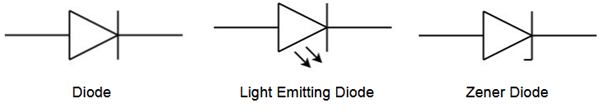
\includegraphics[width=0.7\textwidth]{diode/figurer/oppgave1.png}
%		\caption{Eksempel på forskjellige diode symboler.}
%		\label{fig:diodeSeeeymb}
%	\end{figure}
\end{solution}
\subsection{Løsningsforslag}
\printsolutions[section]

\newpage

\section{Transistor - BJT}
\label{sec:tranBJT}

\subsection{Oppgaver}
%\SetupExSheets{headings=block}

% ------------------ MALER ------------------
\begin{comment}

\begin{question}[name=Oppgave, topic=transBJT]

	\begin{enumerate}[label=\roman*)]

	\end{enumerate}
\end{question}

\vspace{0.5cm} % Add space after the solution

\begin{solution}[name=Løsningsforslag oppgave]

	\begin{figure}[H]
		\centering
		\includegraphics[width=0.7\textwidth]{}
		\caption{}
		\label{fig:}
	\end{figure}
\end{solution}

\vspace{0.5cm} % Add space after the solution
\end{comment}

\begin{question}[name=Oppgave, topic=transBJT]
	\begin{enumerate}[label=\roman*)]
		\item Hva heter de tre tre forskjellig strømmene i en BJT-transistor?
		\item Hvilken av strømmene i en BJT-transistor er vanligvis den største?
		\item Hva er forskjellen mellom saturation og cut-off for en transistor?
		\item Hva beskriver strømforsterkningen $B$?
	\end{enumerate}

\end{question}

\vspace{0.5cm} % Add space after the solution

\begin{solution}[name=Løsningsforslag oppgave]
		\begin{enumerate}[label=\roman*)]
		\item Kollektor-strøm, emitter-strøm og basis-strøm
		\item Emitter er vanligvis den største siden den er summen av kollektor og basestrømmen
		\item Saturation oppstår når transistoren leder maksimalt og spenningsfallet mellom kollektor og emitter er $\approx 0 [V]$.
		
		Cut-off oppstår når det ikke går noen kollektor-strøm og nesten hele det maksimale spenningsfallet ligger over transistorens kollektor og emitter pinner.
		\item Forholdet mellom kollektor-strømmen og base-strømmen.
	\end{enumerate}

\end{solution}

\vspace{0.5cm} % Add space after the solution


\begin{question}[name=Oppgave, topic=transBJT]
Basert på kretsen presentert i Figur \ref{fig:tranBJT1} Beregn verdiene for $I_B$, $I_C$, $I_E$ og $U_{CE}$. Anta en strømforsterkning $\beta =75$ og spenningsfall $U_{BE}=0,7[V]$.

	\begin{figure}[H]
		\centering
		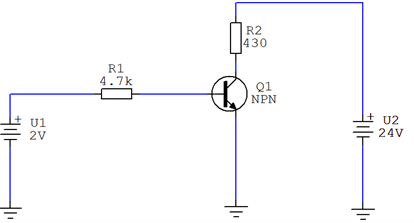
\includegraphics[width=0.7\textwidth]{transistor-BJT/figurer/krets1.png}
		\caption{Krets med BJT-transistor}
		\label{fig:tranBJT1}
	\end{figure}

\end{question}

\vspace{0.5cm} % Add space after the solution

\begin{solution}[name=Løsningsforslag oppgave]
Finner først basis-strømmen.
\[I_B=\frac{U_1-U_{BE}}{R_1}=\frac{2-0,7}{4,7\cdot 10^3}\approx 0,277 [mA]\]

Bruker strømforsterkningen $ \beta $ for å finne strømmen $I_K$.
\[\beta=\frac{I_C}{I_B} \rightarrow I_C= \beta \cdot I_B=75\cdot0,277 \cdot10^{-3} \approx 20,7[mA]\]


Finner så strømmen  $I_C$.
\[I_B+I_C+I_E=0 \rightarrow I_C=I_E-I_B=20,7\cdot 10^{-3} - 0,277 \cdot 10^{-3} \approx 20,42 [mA]\]

Beregner spenningsfallet $U_{BE}$.
\[U_{CE}=U_2-U_{R2}=U_2-(R_2 \cdot I_C) =24-(430 \cdot 20,42 \cdot 10^{-3}) \approx 15,2[V]\]
	
\end{solution}

\vspace{0.5cm} % Add space after the solution

\begin{question}[name=Oppgave, topic=transBJT]
	Basert på kretsen presentert i Figur \ref{fig:tranBJT2} Beregn verdiene for $I_B$, $I_C$, $I_E$ og $U_{CE}$. Anta en strømforsterkning $\beta=250$ og spenningsfall $U_{BE}=0,7[V]$.
	
	\begin{figure}[H]
		\centering
		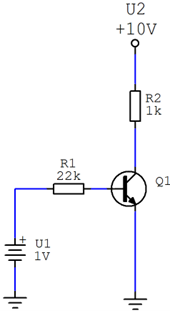
\includegraphics[width=0.25\textwidth]{transistor-BJT/figurer/krets2.png}
		\caption{Krets med BJT-transistor}
		\label{fig:tranBJT2}
	\end{figure}
	
\end{question}

\vspace{0.5cm} % Add space after the solution

\begin{solution}[name=Løsningsforslag oppgave]
Finner basis-strømmen.
\[I_B=\frac{U_{R1}}{R_1}= \frac{1-0,7}{22 \cdot 10^3} \approx 13,64 [\mu A]\]
Bruker transistorens formel for strømforsterkning til å finne emitter-strømmen.
\[I_E=\beta \cdot I_B =250 \cdot 13,64 \cdot 10^{-6} \approx 3,41 [mA]\]

Den relativt store forsterkningen gjør at antall desimaler brukt i $I_B$ vil påvirke nøyaktigheten på $I_E$ i stor grad.

I dette tilfellet er $I_K >>\footnote{Tegnet betyr mye større enn. Eksempel: $9\cdot10^{9}>>1\cdot10^{-10}$} I_B$ og vi kan derfor forenkle beregningen ved å anta $I_E = I_K$

\[U_{CE} = U_2-U_{R_{2}}=10-(1\cdot 10^3 \cdot 3,41 \cdot 10^{-3}) = 6,59 [V] \]


\end{solution}
\vspace{0.5cm} % Add space after the solution
\begin{question}[name=Oppgave, topic=transBJT]
	Basert på kretsen presentert i Figur \ref{fig:tranBJT3} Beregn verdiene for $I_C$, $I_E$, $U_B$ og $U_{BE}$. Anta spenningsfall $U_{BE}=0,7[V]$.
	
	\begin{figure}[H]
		\centering
		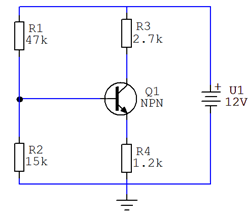
\includegraphics[width=0.45\textwidth]{transistor-BJT/figurer/krets3.png}
		\caption{Krets med BJT-transistor}
		\label{fig:tranBJT3}
	\end{figure}
	
\end{question}

\vspace{0.5cm} % Add space after the solution

\begin{solution}[name=Løsningsforslag oppgave]
Finner spenninging $U_B$

\[U_B= \left(\frac{R_2}{R_1+R_2} \right) \cdot U_1 = \left(\frac{15 \cdot 10^3}{47 \cdot 10^3 + 15 \cdot 10^3} \right) \cdot 12 = 2,9 [V]\]

Beregner emitterspenningen basert på spenningsfallene  $U_B$ og $U_{BE}$.
\[U_E = U_B - U_{BE}=2,90-0,7=2,2 [V]\]

\[I_E = \frac{U_4}{R_4}=\frac{2,2}{1,2 \cdot 10^3} \approx 1,833 [mA]\]

Antar $I_C = I_E$.

Finner totale spenningsfallet fra kollektor-pinnen til jord. Dette er summen av to spenningsfall $U_{CE}$ og $U_{R_{4}}$.
\[U_C = U_1-U_{R_{3}}=U_1-(I_C \cdot R_3)=12-(1,833 \cdot 10^{-3} \cdot 2,7 \cdot 10^{3})=7,1 [V]\]

Trekker fra spenningsfallet over $U_{R_{4}}$ fra $U_C$ for å finne spenningsfallet over transistoren $U_{CE}$.

\[U_{KE} = U_K-U_E=7,1-2,2=4,9 [V]\]

\end{solution}

\vspace{0.5cm} % Add space after the solution


\begin{question}[name=Oppgave, topic=transBJT]
	Basert på kretsen presentert i Figur \ref{fig:tranBJT4} Beregn verdiene for $I_B$, $I_C$, $I_E$ og $U_C$. Anta spenningsfall $U_{BE}=0,7[V]$ og $\beta=90$.
	
	\begin{figure}[H]
		\centering
		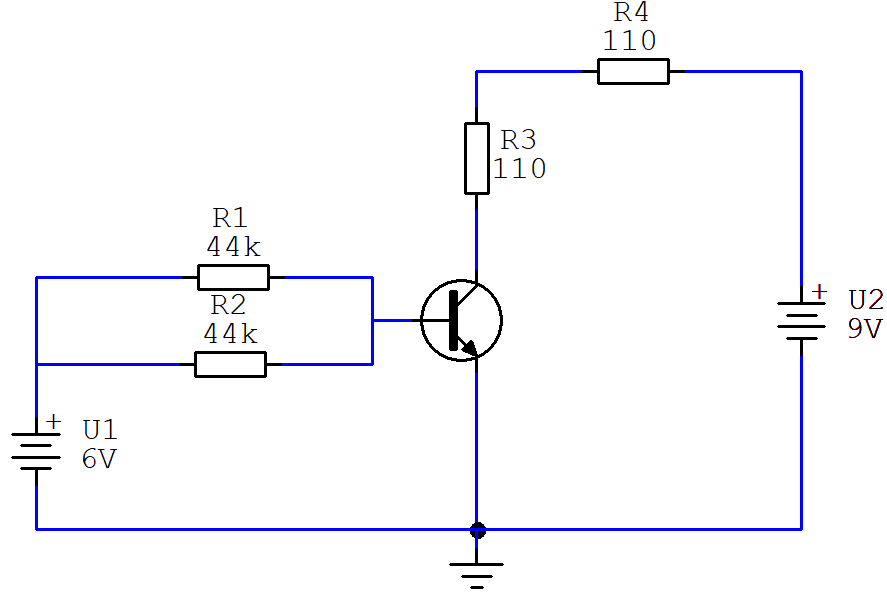
\includegraphics[width=0.6\textwidth]{transistor-BJT/figurer/krets4.png}
		\caption{Krets med BJT-transistor}
		\label{fig:tranBJT4}
	\end{figure}
	
\end{question}

\vspace{0.5cm} % Add space after the solution

\begin{solution}[name=Løsningsforslag oppgave]
Beregner resistansen for basis-strømmen.

\[R_B= \left(\frac{1}{R_1} + \frac{1}{R_2} \right)^{-1} = \left( \frac{1}{44\cdot 10^3} + \frac{1}{44 \cdot 10^3}\right)^{-1}= 22 [k\Omega]\]

Finner $I_B$.

\[I_B = \frac{U_1-U_{BE}}{R_B} = \frac{9-0,7}{22 \cdot 10^3} \approx 0,377 [mA]\]

Bruker forsterkningen $\beta$ til å finne $I_E$.

\[I_E = \beta \cdot I_B = 90 \cdot 0,377 \cdot 10^{-3} \approx 34 [mA] \]

\[I_C = I_C - I_B = 34 \cdot 10^{-3} - 0,377 \cdot 10^{-3} = 33,623 [mA]\]

Finner spenningen $U_C$ som er spenningsfallet mellom kollektor-pinnen og jord.

Summerer kollektor-motstandene
\[R_K = R_3+R_4=110+110=220 [\Omega]\]

\[U_C=U_2-U_{R_{K}} = U_2 - \left( R_K \cdot I_K \right)=9- \left( 220 \cdot 33,623 \cdot 10^{-3} \right) \approx 7,4 [V]\]

\end{solution}

\vspace{0.5cm} % Add space after the solution

\begin{question}[name=Oppgave, topic=transBJT]
	Basert på kretsen presentert i Figur \ref{fig:tranBJT5} Finn motstandsverdien for $R_1$ slik at strømmen i $I_C=120 [mA]$. Anta spenningsfall $U_{BE}=0,7[V]$ og $\beta=96$.
	
	\begin{figure}[H]
		\centering
		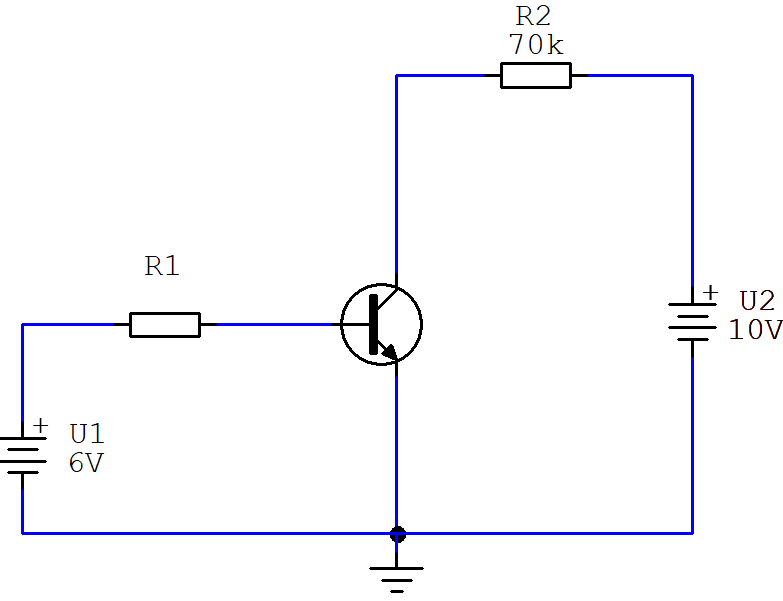
\includegraphics[width=0.6\textwidth]{transistor-BJT/figurer/krets5.png}
		\caption{Krets med BJT-transistor}
		\label{fig:tranBJT5}
	\end{figure}
	
\end{question}

\vspace{0.5cm} % Add space after the solution

\begin{solution}[name=Løsningsforslag oppgave]
\[\beta = \frac{I_C}{I_B} \rightarrow I_B = \frac{I_C}{\beta} \rightarrow I_B= \frac{120 \cdot 10^{-3}}{96} = 1,25[mA]\]

\[R_1= \frac{U_{R_{1}}}{I_B} = \frac{6-0,7}{1,25 \cdot 10^{-3}}=4,24[k\Omega] \]

\end{solution}

\vspace{0.5cm} % Add space after the solution

\begin{question}[name=Oppgave, topic=transBJT]
	
Finn motstandsverdiet for $R_B$ og $R_K$ for kretsen presentert i Figur \ref{fig:tranBJT6}.
	
Kretsen skal dimensjoneres til å ha følgende verdier:
\[U_{KE}=6[V]\]
\[U_{BE}=0,7[V]\]
\[I_K=6[mA]\]

Transistoren $Q_1$ har oppgitt $ \beta= 150$ og spenningen for kilden $ U_b=12[V]$
	
	\begin{figure}[H]
		\centering
		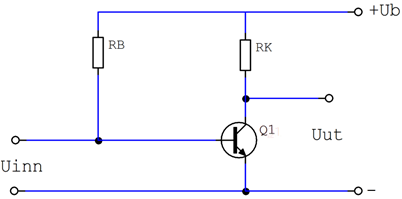
\includegraphics[width=0.6\textwidth]{transistor-BJT/figurer/krets6.png}
		\caption{Krets med BJT-transistor}
		\label{fig:tranBJT6}
	\end{figure}
	
\end{question}

\vspace{0.5cm} % Add space after the solution

\begin{solution}[name=Løsningsforslag oppgave]
\[\beta = \frac{I_C}{I_B} \rightarrow I_B=\frac{I_K}{\beta}=\frac{6 \cdot 10^{-3}}{150} = 40[\mu A]\]

\[R_B=\frac{U_B-U_{BE}}{I_B}= \frac{12-0,7}{40 \cdot 10^{-6}}=282,5[k\Omega] \]

\[R_K=\frac{U_B-U_{KE}}{I_K}= \frac{12-6}{6 \cdot 10^{-3}}=1[k\Omega]\]

\end{solution}


\begin{question}[name=Oppgave, topic=transBJT]
Ta utgangspunkt å Figur \ref{fig:tranBJT7}. Det er brudd i $R_1$. Hva blir verdien for $U_B$, $U_E$ og $U_C$?

	\begin{figure}[H]
		\centering
		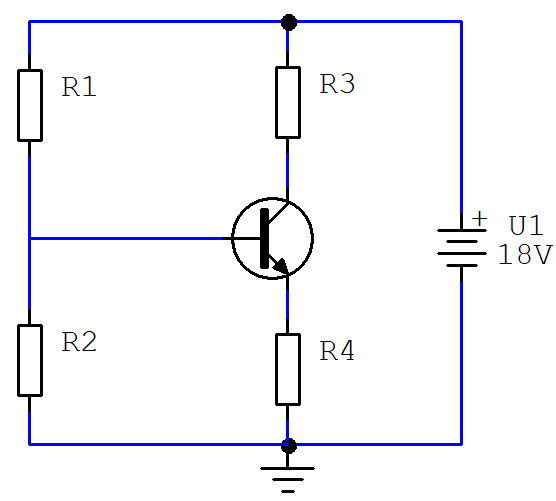
\includegraphics[width=0.5\textwidth]{transistor-BJT/figurer/krets7.png}
		\caption{Krets med BJT-transistor}
		\label{fig:tranBJT7}
	\end{figure}
	
\end{question}

\vspace{0.5cm} % Add space after the solution

\begin{solution}[name=Løsningsforslag oppgave]
	$U_B=0[V]$, $U_E=0[V]$ og $U_C=18[V]$
	Her vil transistoren være i cut-off. Det vil ikke gå noen strøm $I_B$ og transistoren vil derfor ikke lede. Hele spenningen til kilden vil ligge over $U_C$.

\end{solution}




\begin{question}[name=Oppgave, topic=transBJT]
Ta utgangspunkt i kretsen som vist i Figur \ref{fig:tranBJT8} og beregn $I_C$, $U_1$, $\beta$ og $R_1$
	
	\begin{figure}[H]
		\centering
		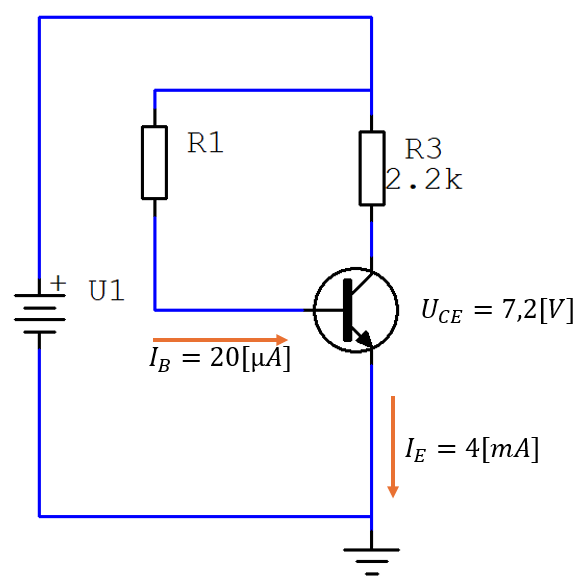
\includegraphics[width=0.5\textwidth]{transistor-BJT/figurer/krets8.png}
		\caption{Krets med BJT-transistor}
		\label{fig:tranBJT8}
	\end{figure}
	
\end{question}

\vspace{0.5cm} % Add space after the solution

\begin{solution}[name=Løsningsforslag oppgave]
\[I_C=I_E - I_C=4 \cdot 10^{-3} - 20 \cdot 10^{-6}= 3,98[mA]\]

\[U_1 = U_{R_C}+U_{CE} = (I_C \cdot R_C)+U_{CE}=(3,98 \cdot 10^{-3} \cdot 2,2 \cdot10^3) + 7,2 = 15,96 [V]\]

\[\beta=\frac{I_C}{I_B}=\frac{3,98 \cdot 10^{-3}}{20 \cdot 10^{-6}}=199\]

\[R_B=\frac{U_B}{I_B}= \frac{15,96-0,7}{20 \cdot 10^{-6}}=763 [k\Omega]\]


\end{solution}
\subsection{Løsningsforslag}
\printsolutions[section]

\newpage



\section{FET transistor}

\section{Forsterker i praksiss}

\section{Måleteknikk}

\newpage

\printbibliography%[title={Referanser}]

\appendix
\chapter[LED Datasheet]{LED Datasheet}
\label{paper-a}

\emph{Datablad fra en standard LED \cite{LEDdatasheet}.}
	
	\bigskip

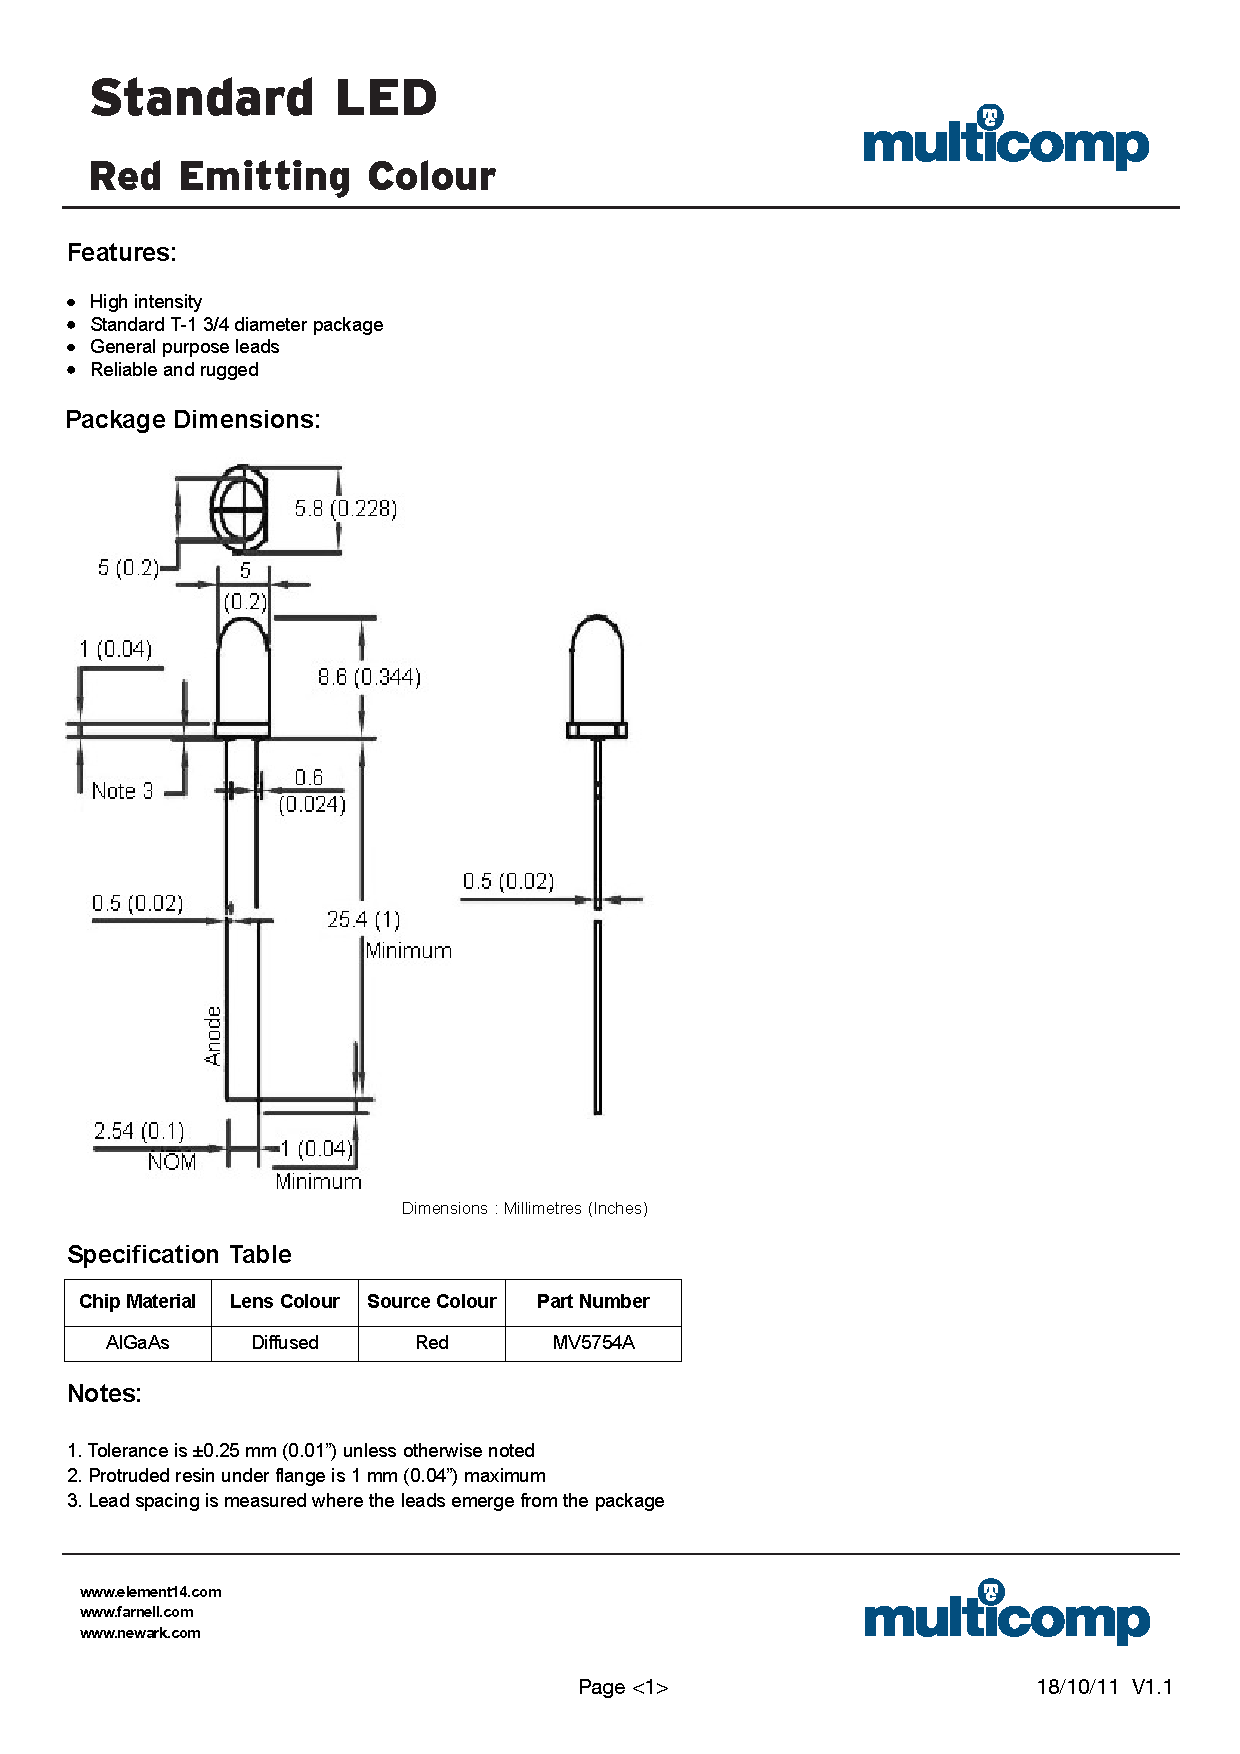
\includepdf[pages=-]{backmatter/pdfVedlegg/1LED_datasheet1498852.pdf}


\end{document}
